\documentclass{article}

\usepackage{amsmath}
\usepackage{listings}
\usepackage{graphicx}      % include this line if your document contains figures
\usepackage{natbib}        % required for bibliography
\usepackage[colorinlistoftodos,prependcaption,textsize=small]{todonotes}
\usepackage[nolist,nohyperlinks]{acronym}
\usepackage{tikz}
\usepackage{float}
\usepackage{mathtools}
\usepackage{pgfplots}
\usepackage{pgfplotstable}
\usetikzlibrary{shapes,arrows, positioning}

\tikzstyle{decision} = [diamond, draw, fill=blue!20, 
    text width=4.5em, text badly centered, node distance=3cm, inner sep=0pt]
\tikzstyle{block} = [rectangle, draw, text centered, ]
\tikzstyle{process} = [block, ]
\tikzstyle{artefact} = [trapezium, draw, text centered, trapezium left angle=120, trapezium right angle=60, ]

\tikzstyle{line} = [draw]
\tikzstyle{arrow} = [draw, -latex']

% \tikzstyle{block} = [triangle, draw, text centered, ]

\definecolor{RYB1}{RGB}{31,  94,  255}
\definecolor{RYB2}{RGB}{255, 31,  94}
\definecolor{RYB3}{RGB}{49,  173, 0}
\definecolor{RYB4}{RGB}{251, 128, 114}
\definecolor{RYB5}{RGB}{128, 177, 211}
\definecolor{RYB6}{RGB}{253, 180, 98}
\definecolor{RYB7}{RGB}{179, 222, 105}


\tikzset{%
  dots/.style args={#1per #2}{%
    line cap=round,
    dash pattern=on 0 off #2/#1
  }
}


\pgfplotsset{compat=1.16}

\title{Rydpair car manual}

\newcommand{\carbrand}{Rydpair}
\newcommand{\carmodel}{rc70}

\newcommand{\emergencyPhoneCost}{5\$}

\author{Car brand}

\begin{document}
    \maketitle

    \section{Safety and Warranty information}
    Please read through and understand the following contents before using your
    new \carbrand{\textregistered} \carmodel{\texttrademark}.
    \carbrand{\textregistered} is not responsible for any physical, emotional,
    material, spectral or other damages to any driver, passenger, mechanic,
    pedestrian, student or other living, undead entity or eldrich horror.

    Should injury occur, the built in phone can be used to dial emergency
    services, however additional charges of \emergencyPhoneCost{} per minute
    may be incurred for the duration of the call.

    \subsection{Seatbelts}

    Before starting the vehicle, all passengers should wear their respective
    seatbelts\footnote{Sold separately}. To use the seatbelts, first ensure
    that the seatbelts are attached properly by tugging on them firmly. Then
    move the metal part attached to the belt to the red and black thingy. The
    metal thingy should attach to the red thingy with an audible click. If the
    audible click is not audible\footnote{this manual is sponsored by. Go to
    audible.com/\carbrand{} for a free audio book} ensure your ears are
    working. If your hearing is indeed working your seatbelts may not be
    installed properly by referring to the installation manual for the
    seatbelts.


    \subsection{In case of fire}

    Step 1: determine what is on fire.

    If the manual is on fire: manually submerge the manual in water.

    If the vehicle is on fire: it is important to remain calm and collected.
    The fire is hot, but not as hot as your mom. With that out of the way, here
    the recommended procedure for dealing with a fire while on the road.


    \begin{enumerate}
        \item{Scream}
        \item{Flail your arms}
        \item{Calm down}
        \item{Exit the vehicle}
        \item{WHAT THE FUCK ARE YOU DOING, THE VEHICLE IS MOVING!}
        \item{Stop the vehicle}
        \item{Exit the vehicle}
        \item{Run for your life}
    \end{enumerate}


    \subsection{Warranty}

    Your \carbrand{} \carmodel{} is under limited warranty. The warranty period is
    one week after date of purchase unless the component damages was caused by
    extraterrestrial events.

    The warranty is void if one of the following has happened
    \begin{itemize}
        \item{Collision with static objects}
        \item{Collision with dynamic objects}
        \item{Exceeding the speed limit}
        \item{Oversteering}
        \item{Understeering}
        \item{Replacement of components with non-manufacturer-approved components}
        \item{Other things which may hamper the performance of the vehicle}
        \item{Reading the rest of the manual before reading Section~\ref{sec:reading_the_manual}
            after reading this
        }
    \end{itemize}

    \twocolumn

    \subsection{Reading this manual}\label{sec:reading_the_manual}

    Before reading this manual, ensure you have read the following section which
    instructs you how to read the manual. The manual is divided into several
    sections, each section starts with a headline which is somewhat related to
    the contents of the corresponding section. A table of content is available
    for additional charge.

    Some sections like the previous section are in single column mode, while the
    current section has two columns. If you had to read the previous section to check
    whether or not it was in single column mode, you did good, as it meant that you
    read Section~\ref{sec:reading_the_manual} before reading the manual. If not,
    you really should pay more attention before reading.

    \onecolumn

    \subsection{Electrical system}

    Not all components are electrically compatible with each other, in particular,
    make sure that your generator does not feed the wrong voltage to the component.
    For details, consult Figure~\ref{fig:generator_flowchart}.

    \begin{figure}
        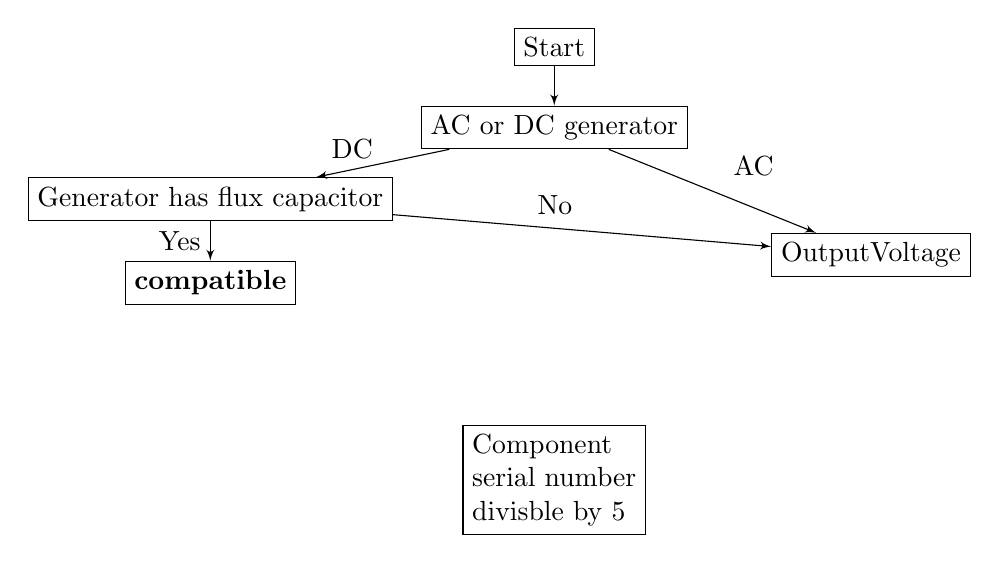
\begin{tikzpicture}[
    auto,
    node distance=0.5cm,
    every label/.style={align=left},
    every node/.style={align=left}
]
    \node[process] (start) {Start};
    \node[process, below = of start] (isAc) {AC or DC generator};

    \node[process, below left = of isAc] (hasFluxCapacitor) {Generator has flux capacitor};
    \node[process, below = of hasFluxCapacitor] (yes1) {\textbf{compatible}};
    \node[process, below right = 1.5cm of isAc] (outputVoltage) {OutputVoltage};

    \node[process, below = 3.5cm of isAc] (5V) {Component\\ serial number\\ divisble by 5};

    \path[arrow] (start) -- (isAc);

    \path[arrow] (isAc)
        -- node [
            midway,
            yshift=0.3cm,
            label=left:{DC}
        ] {}
        (hasFluxCapacitor);
    \path[arrow] (isAc)
        -- node [
            midway,
            yshift=0.2cm,
            xshift=0.9cm,
            label=left:{AC}
        ] {}
        (outputVoltage);

    \path[arrow] (hasFluxCapacitor)
        -- node [
            midway,
            label=left:{Yes}
        ] {}
        (yes1);

    \path[arrow] (hasFluxCapacitor)
        -- node [
            midway,
            yshift=0.2cm,
            label=left:{No}
        ] {}
        (outputVoltage);
\end{tikzpicture}

        \caption{Determining if a component is compatible with a
        generator}\label{fig:generator_flowchart}
    \end{figure}
\end{document}
